\chapter{Prerequisites}
\label{chap:02_prerequisites}

For the whistle sound source localization with multiple robots, some
sequential steps needs to interact for a final result.
To work with the implementations in \cref{chap:03_implementation}, the fundamentals
are introduced in this chapter on a general basis.

As this work specializes on the localization of a whistle sound, this sound pattern
must be detected at first.
This was already done by previous work \cite{Hasselbring}.
Hence, the flow of the whistle detection are briefly explained in \cref{sec:02_whistleSignal}.
The position of the sound source is determined by combining the
separate direction results on the single robots.
Utilizing the \ac{TDOA} information as in \cref{sec:02_tdoa} between the pairs
of the Naos' microphones, every robot produces a sound direction ray which
are feed into the team decision filter.
As mentioned in \cref{chap:01_introduction}, different methods exist to identify the \ac{TDOA}
and are terms of content in \cref{sec:02_cc,sec:02_gcc,sec:02_phase}.
Due to the low resolution arising from the sample rate and the distance between the microphones,
a subsample estimation is used based on \cref{sec:02_subsampleShift}.
One of the most significant factors is the selection of the signal frame that is used for
the direction determination.
In order to provide a correct and stable decision process, the different approaches to
consider are shortly mentioned in \cref{sec:02_signalStartDetection}.
After all, the results of the individual robots are filtered by assuming
gaussian distribution to produce a sound source position.
By passing information about the certainty of the single robot result, the
filtering explained in \cref{sec:02_filter} is related to a Kalman filter without
prediction step.

% \missing[]{
% - CC in time domain, because low frequency resolution (44100Hz/512samples=resolution)\\
% and also CC corrupted and we want to detect which signal was first\\
% }

\section{Whistle Signal}
\label{sec:02_whistleSignal}

In this work the localization of a whistle sound source is to be to the fore.
The detection of such a signal is implemented as stated in \cite{Hasselbring}.\\
- short explanation of how the whistle is detected\\
- whistle sound is around 2000Hz and 4000Hz

Further on, the mathematical model of a received whistle signal at one microphone sensor
is defined as
\be
x(t) = s(t) + n(t)
\label{eq:02_whistleSignal}
\ee
where $s(t)$ represents the signal and $n(t)$ noise.
Both are real, jointly stationary random processes.
\section{Time Difference Of Arrival}
\label{sec:02_tdoa}

The direction of a signal source $\gamma'$ can be detected by the time delay of
the received signal.
Calculations for the direction of the sound source can be done with a
geometrical approach like in \cite{Valin_Michaud}.
\Cref{fig:02_tdoa} illustrates the delay introduced by the direction angle
of the sound source relative to a vector between channels 0 and 1.
If the delay is zero, the signal is perpendicular to this channels vector.
It's value can be $s_{max}$ maximally which delivers the result that the source
direction must be aligned to the channels vector direction.
It is assumed that the distance from the sensors to the sound source is
significantly large so that the signal waves proceed parallel which is a necessary
criterion for the approach to be valid.
\begin{figure}[ht]
	\centering
		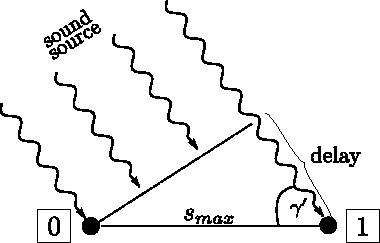
\includegraphics[width=0.4\columnwidth]{figures/tdoa_waves}
	\caption{Illustration of TDOA principle.}
    \label{fig:02_tdoa}
\end{figure}
% -------------------------------------------------------------

Specifying the speed of sound $c_s$ being 343\si{m/s} in air, the angle
$\gamma'$ can be defined as
\bsub \bal
    \gamma' &= cos^{-1}(\frac{|delay|}{s_{max}})
    \label{eq:02_tdoaAngle}\\
    \intertext{with}
    s_{max} &= \frac{f_s * d_{max}}{c_s}
\eal \esub
where $f_s$is the sampling rate.
% -------------------------------------------------------------

With the definition of a whistle signal as stated in \cref{eq:02_whistleSignal},
the microphone sensors $mic_1$ and $mic_2$ will output
\bsub \bal
    x_1(t) &= s(t) + n_1(t)\\
    x_2(t) &= \alpha s(t - D) + n_2(t).
\eal \esub
\label{eq:02_signalTimeDomain}
Here, $D$ is the delay of $x_2$ relative to $x_1$ for which is looked for.
\section{Cross Correlation}
\label{sec:02_cc}

The \ac{CC} provides information about the similarity of two signals.
Thus, the delay of one signal can be detected where the \ac{CC} function $R_{x_0x_1}(t)$ is largest.
% -------------------------------------------------------------
In time domain, the \ac{CC} of two signals $x_0$ and $x_1$ is denoted as
\bal
    R_{x_0x_1}(t) = \int^{+\infty}_{-\infty}x_0(\tau-t)x_1(\tau)d\tau.
\eal
Considering the frequency domain, the function can be transformed into
\bal
    \mathcal{F}[R_{x_0x_1}(t)] = G_{x_0x_1}(f) = X_0^*(f)X_1(f)
    \label{eq:02_ccBaseFunction}
\eal
with $\mathcal{F}[x_i(t)] = X_i(f)$ and $X_i^*(f)$ indicating the conjugate complex form.
% -------------------------------------------------------------
However, the finite observation time of the received signal corrupts the fourier
transform \cite{K_C_GCC}
and noise of sensors may introduce false peaks in the \ac{CC} \cite{H_B_GCC}.
% -------------------------------------------------------------
In frequency domain, the signals $x_0(t)$ and $x_1(t)$ from \cref{eq:02_signalTimeDomain}
can be expressed as
\bsub
\label{eq:02_signalFreqDomain}
\bal
    X_0(f) &= S(f) + N_0(f)\\
    X_1(f) &= \alpha S(f) e^{-j2\pi fD}+ N_1(f).
\eal \esub
% -------------------------------------------------------------
Thus, the \ac{CC} is
\bsub
\label{eq:02_Gx0x1}
\bal
    G_{x_0x_1}(f) &= \alpha |S(f)|^2 e^{-j2\pi fD} + N_0^*(f)N_1(f) + S^*(f) N_1(f) + \alpha S(f) e^{-j2\pi fD}N_0^*(f)\\
\intertext{which will be shortened as}
    G_{x_0x_1}(f) &= \alpha \phi_s(f) e^{-j2\pi fD} + \phi_n(f) + \phi_c(f) \label{eq_02_Gx0x1_simple} \\
\intertext{where}
\phi_s(f) &= |S(f)|^2 \label{eq:02_phi_s} \\
\phi_n(f) &= N_0^*(f)N_1(f) \label{eq:02_phi_n1n2} \\
\phi_c(f) &= S^*(f) N_1(f)+\alpha S(f)e^{-j2\pi fD}N_0^*(f) \label{eq:02_phi_c}.
\eal \esub
%\cite{H_B_GCC}
% -------------------------------------------------------------
Considering the ideal case where $s(t)$, $n_0(t)$ and $n_1(t)$ are uncorrelated, the terms
$\phi_c$ and $\phi_n$ disappear and the \ac{CC} results in
\bal
    R_{x_0x_1}(t) = \mathcal{F}^{-1}[\alpha \phi_s(f) e^{-j2\pi fD}] = \alpha \mathcal{F}^{-1}[\phi_s(f)] * \delta(t-D).
    \label{eq:02_R12_noNoise}
\eal
In general, $\phi_c$ and $\phi_n$ can neither be neglected nor assumed as uncorrelated to the signal \cite{H_B_prob},
so that they introduce inaccuracies and errors.

% -------------------------------------------------------------
% \unsure[]{do I fully understand this? Is this correct?}
% This means there exists a peak at delay $D$ which is altered by the \ac{iFT}
% of the signal spectrum.
As introduced, the \ac{CC} gives insight about the similarity of two signals and at peak, they
are most alike.
Received signals from microphone sensors are digital signals sampled with a certain
frequency.
The derivations are just as applicable, but transformations into frequency
domain are done by \ac{DFT}.
In the case of real data samples with length $n$ and similar \ac{DFT} size, the shift between
the zero index and the peak is the resulting delay $D$.
Zero index is defined as the index of the peak if no shift exists.
% -------------------------------------------------------------

\Cref{fig:03_ccTheory} is the outcome of two similar, but shifted sine signals with
3\si{\kilo\hertz} and normally distributed noise.
As the second signal is delayed by 10 samples, the peak can be detected where $shift = 10$.
The example signals are attached in \cref{fig:ap1_signals}.
One disadvantage of this technique is that for periodic signals the \ac{CC} also is periodic
and the peak is not always easily detectable. Noise and inaccuracies of the \ac{FFT} then
may influence the result what can make the peak unobvious \cite{L_L_GCC}.
\begin{figure}[ht]
	\centering
		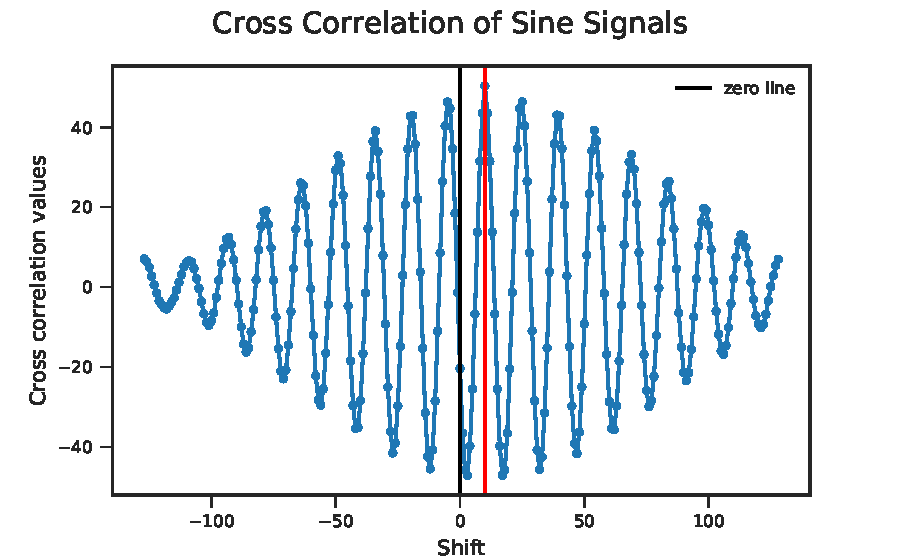
\includegraphics[width=1\columnwidth]{figures/CC_theory}
	\caption{Cross correlation of two generated sine signals with 3\si{\kilo\hertz}.}
    \label{fig:03_ccTheory}
\end{figure}

\section{Generalized Cross Correlation}
The generalized cross correlation is super duper nice.

\section{Signal Phase Difference}
\label{sec:02_phase}

With a different approach to the correlation methods, the \ac{TDOA} can be
detected by observing the phase of one reference frequency $f_c$.
Imaging a single-sinusoidal signal moving from left to right as
pictured in \cref{fig:02_phaseTheory}, two distant sensors
(\textit{channel 2} and \textit{channel 3}) will
receive different parts of the signal at the same time.
Transforming the frames into frequency domain by \ac{FFT}, the pase of the
maximal frequency differ by the delay.
% -------------------------------------------------------------

\begin{figure}[ht]
	\centering
		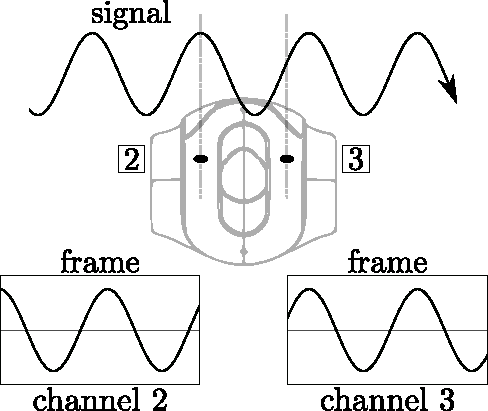
\includegraphics[width=0.35\columnwidth]{figures/phase_theory}
	\caption{Explanatory illustration of the phase difference method.}
    \label{fig:02_phaseTheory}
\end{figure}
% -------------------------------------------------------------

The phase of a signal's reference frequency is easily computable in frequency domain
with
\bal
    \phi(f_c) &= tan^{-1}\left(\frac{imag(X(f_c))}{real(X(f_c))}\right).
\eal
% -------------------------------------------------------------
With the difference of the phases of two channel, the delay in meters is defined as
\bal
    D &= \frac{\Delta \phi \cdot c_s}{2 \pi \cdot f_c}.
\eal
From that, the direction angle calculation of \cref{eq:02_tdoaAngle} can
be followed.
It should be noted that certain requirements needs to be fulfilled to receive a
unambiguous result due to signal periodicity.
\Cref{subsubsec:03_phase} covers the conditions that apply for this thesis's
hardware.
% -------------------------------------------------------------
\section{Subsample Shift}
\label{sec:02_subsampleShift}

Considering the case that the sample frequency $f_s$ is set to 44.1\si{\kilo\hertz}
and the sound speed is 343\si{m/s}, the maximum number of samples
between the rear channels is 14.
Other neighboring pairs have even less maximum sample differences.
This leads to a very low resolution of the direction angle which can be
circumvented by either setting a higher resolution or interpolation.

Quadratic interpolation is a well known technique to obtain a floating number
shift from a correlation.
For this, a parabola $y(x) = a(x-p)^2+b$ is fitted into the three values of $R$ around the peak
of the \ac{CC} and the peak of the parabola is taken as the more accurate
delay.
Thus, the subsample delay $D_{sub}$ depends on the maximum value of the correlation $y_m$
and its previous one $y_{m-1}$ and the next value $y_{m+1}$.
Substituting known values and derivations into the parabola function,
the subsample delay is defined as
\bal
	D_{sub} = \frac{y_{m-1} - y_{m+1}}{2 \cdot (y_{m-1} - 2y_{m} + y_{m+1})}
	\label{eq:02_subsample}
\eal
like in \cite{C_H_subsampleDelay}.
% -------------------------------------------------------------
\Cref{fig:02_subsampleShift} illustrates the \ac{CC} of two generated sine signals with 3\si{\kilo\hertz}.
The second signal is shifted by $\frac{\pi}{3}$ which are 2.449 samples for a sample rate
of 44.1kHz.
As the plot shows, the peak of the parabola can be determined at an index of 2.446 by
quadratic interpolation.
\begin{figure}[ht]
	\centering
		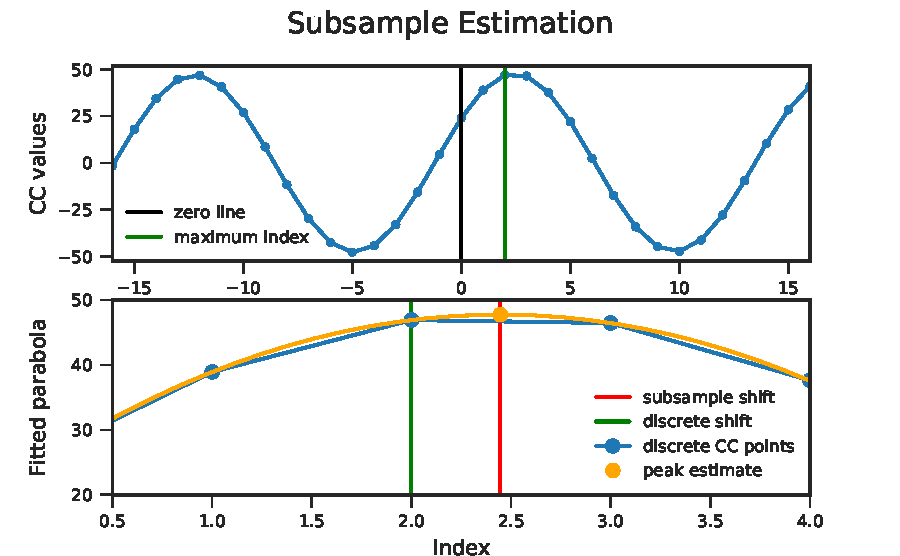
\includegraphics[]{figures/subsample_shift}
	\caption{Explanation example of the subsample shift estimation using parabolic interpolation.}
    \label{fig:02_subsampleShift}
\end{figure}
% -------------------------------------------------------------
In research there are efforts in finding a better approximation function than the quadratic as stated
in \cite{S_L_subsampleInterpolation} but these are not discussed in greater detail here
due to sufficiency.
% -------------------------------------------------------------
% index = 2 -> -14.6deg
% index = 3 -> -22.2deg
% index = 2.445 -> -17.9deg
\section{Signal Start Detection}
\label{sec:02_signalStartDetection}

One focus of the whistle signal localization is the correct choice of the
signal frame, with which the \ac{TDOA} measurement is done.
In order to perform the \ac{FFT} most efficiently, the size of one frame
should be a power of 2.
Assuming that the clearest signal without reverberation and with minimal
multipath propagated subsignals is at the start of a sound signal,
the frame to investigate is chosen to be at the beginning of a whistle sound.
Several methods exist and can be combined at will.
In the next subsections, signal start detection using entropy, energy and
zero crossing rate are subject of discussion.

\subsection{Entropy}
\section{Spectral Subtraction}
\label{sec:02_spectralSubtraction}

\section{Bayesian Updating}
\label{sec:02_filter}

Assuming gaussian distribution of the single robot results,
the multi-agent decision process is done by Bayesian Updating.
One dimensional probability density functions of states with
variance $\sigma^2$ and mean $\mu$ are described as
\bal
    \mathcal{N}(x,\sigma,\mu) = \frac{1}{\sigma\sqrt{2\pi}}e^{-\frac{(x-\sigma)^2}{2\sigma^2}}.
    \label{eq:02_probabilityDensity}
\eal
Having two values $\mu_0$ and $\mu_1$ with their variances,
the result $\mu'$ of the combination of both is
\bal
    \mathcal{N}(x,\sigma',\mu') = \mathcal{N}(x,\sigma_0',\mu_0') \cdot \mathcal{N}(x,\sigma_1',\mu_1').
    \label{eq:02_newProbabilityDensity}
\eal
By substitution and conversion, $\mu'$ and $\sigma'^2$ can be
formulated to
\bsub
\label{eq:02_intersectionState}
\bal
    \mu' &= \mu_0 + \frac{\sigma_0^2(\mu_1-\mu_0)}{\sigma_0^2+\sigma_1^2}\\
    \sigma'^2 &= \sigma_0^2 - \frac{\sigma_0^4}{\sigma_0^2+\sigma_1^2}.
\eal
\esub

\subsection{Two Dimensional Case}
\label{subsec:02_2dTeam}

Imaging having results from two agents that accomplished the \ac{WSDE} algorithm by
computing the \ac{TDOA} with any method, either the \ac{WSDE} angles of both robots
cross and an intersection point would be found or no final whistle source position result arises.
Each of these intersection points can be interpreted as whistle source positions
with given state $\mu$ and variance $\sigma$ of \cref{eq:02_probabilityDensity}.
Final whistle source position of all robots is estimated by iterating over
all intersections and updating the result with \cref{eq:02_intersectionState}.

Exemplary, two robots at position $\vec{p_j}$ and $\vec{p_k}$ with their \ac{WSDE} results
are illustrated in \cref{fig:03_rays}.
\begin{figure}[ht]
	\centering
		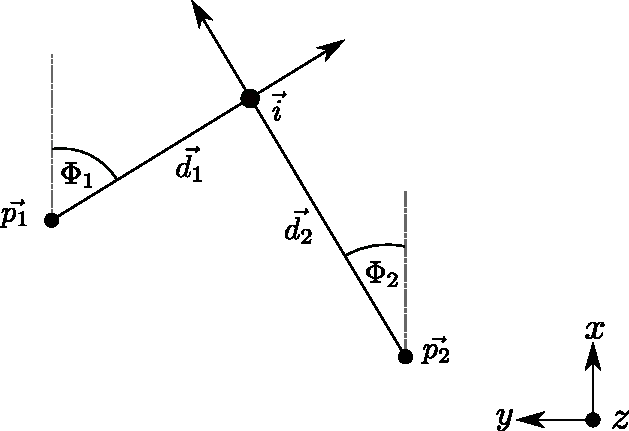
\includegraphics[width=0.50\textwidth]{figures/rays}
    \caption[Nomenclature for multi-agent localization algorithm]
            {Nomenclature for multi-agent localization algorithm.}
    \label{fig:03_rays}
\end{figure}
% -------------------------------------------------------------

Every \ac{WSDE} result is represented as \textit{ray} which consists of the robot position
$\vec{p_j}$ and the \ac{WSDE} angle $\Phi_j$, both in field coordinates.
The \ac{WSDE} angle $\gamma_j$ is defined relative to the robot and the robot's orientation $\theta_j$
is known by its team message information.
Thus, the absolute angle is
\bal
\Phi_j &= \theta_j + \gamma_j\\
\intertext{from which the whistle source direction ray can be described as}
\vec{r_j} &= \vec{p_j} + \vec{d_j} % = \begin{pmatrix}p_{jx}\\p_{jy}\end{pmatrix} + \ell \begin{pmatrix}d_{jx}\\d_{jy}\end{pmatrix}
    = \begin{pmatrix}p_{jx}\\p_{jy}\end{pmatrix} + \ell \begin{pmatrix}\cos(\Phi_j)\\\sin(\Phi_j)\end{pmatrix}.
\label{eq:03_ray}
\eal

An intersection point of two rays $\vec{r_j}$ and $\vec{r_k}$ is expressed as
\bal
    \vec{i_{jk}} &= \begin{pmatrix}i_{jkx}\\i_{jky}\end{pmatrix}
\eal
with x- and y-coordinates.
If two real numbers $u$ and $v$ exist, so that
\bal
    \vec{i_{12}} &= \vec{p_1} + u \cdot \vec{d_1} = \vec{p_2} + v \cdot \vec{d_2}
    \label{eq:03_intersection}
    \\
    \intertext{a intersection point can be determined by simple geometrical relations.
               With the given terms and conditions $u$ and $v$ values are computed by
               dividing the vectors into x- and y-value and solving the equations, resulting in}
    u &= \frac{p_{1y} \cdot d_{2x} + d_{2y} \cdot p_{2x} - p_{2y} \cdot d_{2x} - d_{2y} \cdot p_{1x}}
            {d_{1x} \cdot d_{2y} - d_{1y} \cdot d_{2x}}
            \label{eq:03_intersectionU}
            \\
    v &= \frac{p_{1x} + d_{1x} \cdot u - p_{2x}}{d_{2x}}.
\eal
% -------------------------------------------------------------

% DEFINITION COVARIANCE MATRIX
The covariance matrix $\textbit{C}_{jk}$ is obtained in the spirit of an Extended Kalman filter \cite{kalman}
considering the Jacobian matrix $\textbit{J}_{jk}(\Phi_j, \Phi_k)$ and the average angle error $\varepsilon_{\Phi}$
over all available measurements.
Expressing the direction vector $\vec{d}_j$ of the ray by angle $\Phi_j$ as in \cref{eq:03_ray}, the covariance
matrix of the intersection of two rays $\vec{r}_j$ and $\vec{r}_k$ is
\bsub
\label{eq:03_cov}
\bal
\textbit{C}_{jk} &= \left( \begin{matrix}
                        \varepsilon_{\Phi} & 0 \\
                        0 & \varepsilon_{\Phi} \\
                      \end{matrix} \right) \cdot \textbit{J}_i(\Phi_j, \Phi_k)
\\
\intertext{with the Jacobian matrix}
\textbit{J}_i(\Phi_j, \Phi_k) &= \left(\begin{matrix}
    \frac{\partial ix}{\partial \Phi_j} & \frac{\partial ix}{\partial \Phi_k} \\
    \frac{\partial iy}{\partial \Phi_j} & \frac{\partial iy}{\partial \Phi_k} \\
    \end{matrix}\right).
\eal
\esub
The elements of the Jacobian result by derivation of the intersection formula \cref{eq:03_intersection}
with \cref{eq:03_intersectionU,eq:03_ray} and yield
\begin{align*}
\frac{\partial ix}{\partial \Phi_1} &= \frac{(\cos(\Phi_2) \cdot (\cos(\Phi_1)^2 + \sin(\Phi_1)^2) \cdot ((p_{1y} - p_{2y}) \cdot \cos(\Phi_2) +
                                  (-p_{1x} + p_{2x}) \cdot \sin(\Phi_2)))}
                                  {(-\cos(\Phi_2) \cdot \sin(\Phi_1) + \cos(\Phi_1) \cdot \sin(\Phi_2))^2}
                                  \\
\frac{\partial ix}{\partial \Phi_2} &= \frac{-(\cos(\Phi_1) \cdot (\cos(\Phi_2)^2 + \sin(\Phi_2)^2) \cdot ((p_{1y} - p_{2y}) \cdot \cos(\Phi_1) + (-p_{1x} + p_{2x}) \cdot \sin(\Phi_1)))}
                                {(\cos(\Phi_1) \cdot \sin(\Phi_2) - \cos(\Phi_2) \cdot \sin(\Phi_1))^2}
                                \\
\frac{\partial iy}{\partial \Phi_1} &= \frac{(\cos(\Phi_1)^2 + \sin(\Phi_1)^2) \cdot \sin(\Phi_2) \cdot ((p_{1y} - p_{2y}) \cdot \cos(\Phi_2) + (-p_{1x} + p_{2x}) \cdot \sin(\Phi_2))}
                                {(-\cos(\Phi_2) \cdot \sin(\Phi_1) + \cos(\Phi_1) \cdot \sin(\Phi_2))^2}
                                \\
\frac{\partial iy}{\partial \Phi_2} &= \frac{(\cos(\Phi_2)^2 + \sin(\Phi_2)^2) \cdot \sin(\Phi_1) \cdot ((-p_{1y} + p_{2y}) \cdot \cos(\Phi_1) + (p_{1x} - p_{2x}) \cdot \sin(\Phi_1))}
                                {(\cos(\Phi_1) \cdot \sin(\Phi_2) - \cos(\Phi_2) \cdot \sin(\Phi_1))^2}.
%  \label{eq:03_jacobianElements}
\end{align*}

